%!TEX root = ../dokumentation.tex

\chapter{Umsetzung}

%title wird unter dem Bsp. abgedruckt
%caption wird im Verzeichnis abgedruckt
%label wird zum referenzieren benutzt, muss einzigartig sein.

\section{Voraussetzungen}
Hier kommt der Scheiß ist zustand rein

\section{Konzept}
Hier kommt der Scheiß ist zustand rein
\begin{figure}[h]
	\centering
	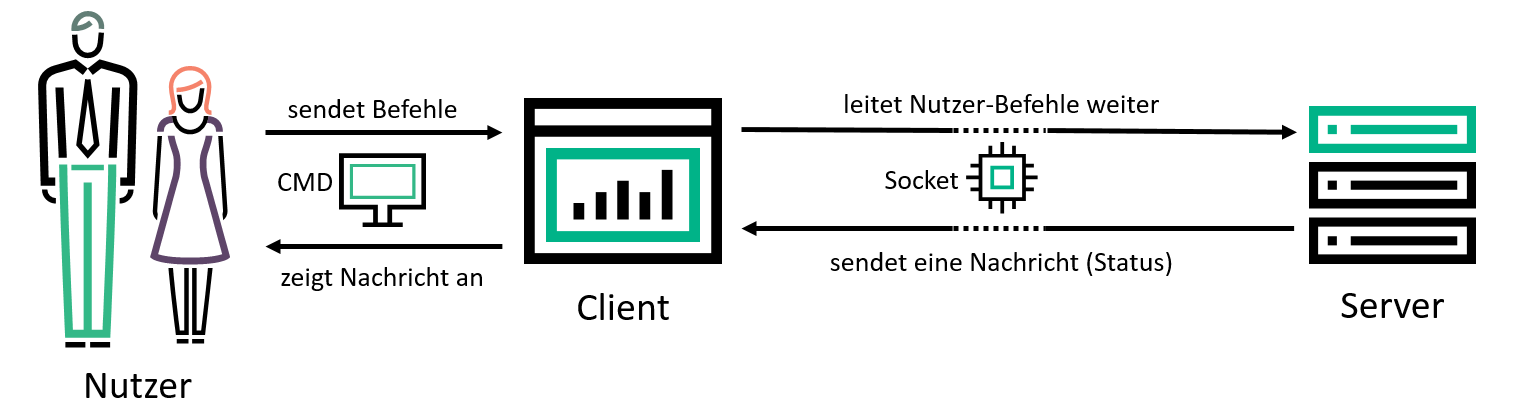
\includegraphics[scale=0.5]{Audioplayer_Konzept.png}
	\caption{Audioplayer - Konzept}
	\label{img:grafik-RaspberryPi3}
\end{figure}
\newline

\section{Kommunikation über Sockets}
Hier kommt der Scheiß ist zustand rein

\section{Funktionen des Programmes}
Hier kommt der Scheiß ist zustand rein

